\documentclass[a4paper,openright,12pt]{book}
\usepackage[spanish]{babel} % espanol
\usepackage{fancyhdr}
\usepackage{lastpage}
\usepackage{graphicx} % graficos
\usepackage{hyperref}
\usepackage[utf8]{inputenc}
\usepackage{enumerate}


% nivel que se numera y aparece en el indice
\setcounter{secnumdepth}{3}
\setcounter{tocdepth}{3}

% quitar el 0.
\renewcommand\thesection{\arabic{section}}

% tabla de contenidos como seccion
\makeatletter
\renewcommand\tableofcontents{
    \section*{{Tabla de contenidos} %linea importante
        \@mkboth{
           \MakeUppercase\contentsname}{\MakeUppercase\contentsname}}
    \@starttoc{toc}
    }
\makeatother

% bibliografia como seccion
\makeatletter
\renewenvironment{thebibliography}[1]{
     \section*{Bibliografía} %linea importante
      \@mkboth{\MakeUppercase\bibname}{\MakeUppercase\bibname}
      \list{\@biblabel{\@arabic\c@enumiv}}
           {\settowidth\labelwidth{\@biblabel{#1}}
            \leftmargin\labelwidth
            \advance\leftmargin\labelsep
            \@openbib@code
            \usecounter{enumiv}
            \let\p@enumiv\@empty
            \renewcommand\theenumiv{\@arabic\c@enumiv}}
      \sloppy
      \clubpenalty4000
      \@clubpenalty \clubpenalty
      \widowpenalty4000
      \sfcode`\.\@m}
     {\def\@noitemerr
       {\@latex@warning{Empty `thebibliography' environment}}
      \endlist}
\makeatother

% aqui definimos el encabezado
\lhead[\thepage/\pageref{LastPage}]{}
\chead[Informe]{Informe}
\rhead[]{\thepage/\pageref{LastPage}}
\renewcommand{\headrulewidth}{0.5pt}

% aqui definimos el pie de pagina
\lfoot[EPIS]{Base de Datos II}
\cfoot[\today]{\today}
\rfoot[Base de Datos II]{EPIS}
\renewcommand{\footrulewidth}{0.5pt}

\pagestyle{fancy} 

% margenes
\setlength{\oddsidemargin}{10mm}
\setlength{\evensidemargin}{10mm}

\begin{document}

\begin{titlepage}
\vspace*{4cm}
\centering
\Huge
\textbf{Cómo hacer un Reporte o Informe con LaTeX} \\
\vspace*{0.8cm}
\rule{80mm}{0.1mm} \\
\vspace*{0.2cm}
\Large
Ariel Marina \\
\vspace*{0.1cm}
\large
\today
\normalsize
\end{titlepage}

\tableofcontents
\pagenumbering{arabic}
\lhead[\thepage/\pageref{LastPage}]{\thesection. Tabla de contenidos}
\rhead[\thesection. Tabla de contenidos]{\thepage/\pageref{LastPage}}
\newpage

\section{Introducción}\label{se:intro}
\lhead[\thepage/\pageref{LastPage}]{\thesection. Introduccion}
\rhead[\thesection. Introduccion]{\thepage/\pageref{LastPage}}

\section{4-1 Ejercicio 0}\label{se:nudo}
\lhead[\thepage/\pageref{LastPage}]{\thesection. Nudo}
\rhead[\thesection. Nudo]{\thepage/\pageref{LastPage}}
\section{4-1 Ejercicio 1}\label{se:nudo}
\lhead[\thepage/\pageref{LastPage}]{\thesection. Nudo}
\rhead[\thesection. Nudo]{\thepage/\pageref{LastPage}}
\section{4-2 Ejercicio 1}\label{se:nudo}
\lhead[\thepage/\pageref{LastPage}]{\thesection. Nudo}
\rhead[\thesection. Nudo]{\thepage/\pageref{LastPage}}
\section{4-2 Ejercicio 2}\label{se:nudo}
\lhead[\thepage/\pageref{LastPage}]{\thesection. Nudo}
\rhead[\thesection. Nudo]{\thepage/\pageref{LastPage}}



\section{5-1 Ejercicio 1: Creación de un Glosario a Partir del Modelo Lógico}\label{se:nudo}
\lhead[\thepage/\pageref{LastPage}]{\thesection. Nudo}
\rhead[\thesection. Nudo]{\thepage/\pageref{LastPage}}
Descripción general\\
En esta práctica, creará un glosario a partir del modelo lógico de la base de datos académica.\\
Tareas

\begin{enumerate}
    \item Abra el modelo lógico de la base de datos académica.
    \item Haga clic con el botón derecho en el nodo Logical Model en el explorador y seleccione "Create Glossary from Logical Model".
    \item Especifique el nombre del glosario, una breve descripción y tantos tipos de clasificación como sean aplicables a las entradas del glosario.
    \item Guarde el glosario.
\end{enumerate}
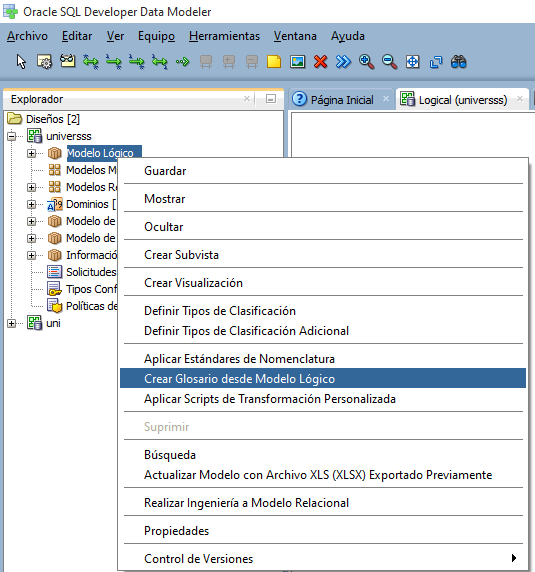
\includegraphics[width=11cm]{./images/5-1 Ejercicio 1/1.png}
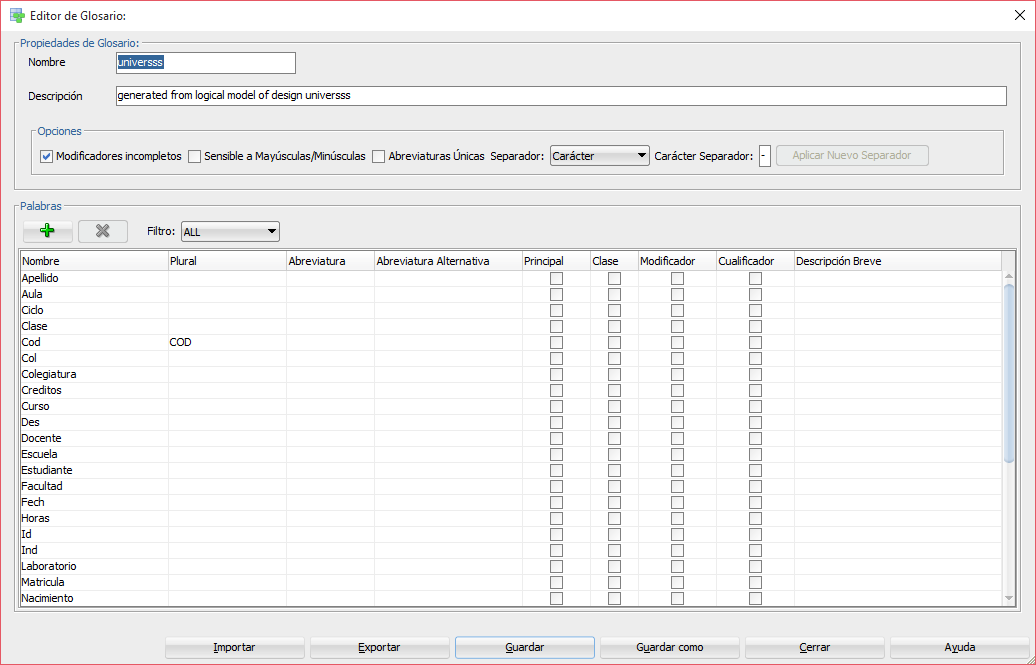
\includegraphics[width=17cm]{./images/5-1 Ejercicio 1/2.png}
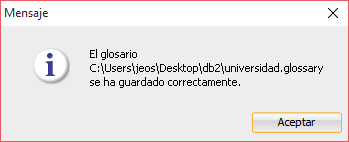
\includegraphics[width=12cm]{./images/5-1 Ejercicio 1/3.png}


\section{5-1 Ejercicio 2: Creación de un Archivo.csv con Nombres Predefinidos}\label{se:nudo}
\lhead[\thepage/\pageref{LastPage}]{\thesection. Nudo}
\rhead[\thesection. Nudo]{\thepage/\pageref{LastPage}}
Descripción general\\
En esta práctica, creará un archivo .csv con abreviaturas de los nombres predefinidos que se utilizarán en el modelo relacional de la base de datos académica.\\
Tareas


\begin{enumerate}
\item  Haga clic en Tools > Name Abbreviations.
\item Especifique el archivo .csv que contiene los pares de valores separados por comas.
\item Especifique los objetos a los que se aplicarían los cambios de nombre.
\item Especifique si se mantendrán las mayúsculas o minúsculas del nombre actual al cambiar la cadena de nombre
\end{enumerate}
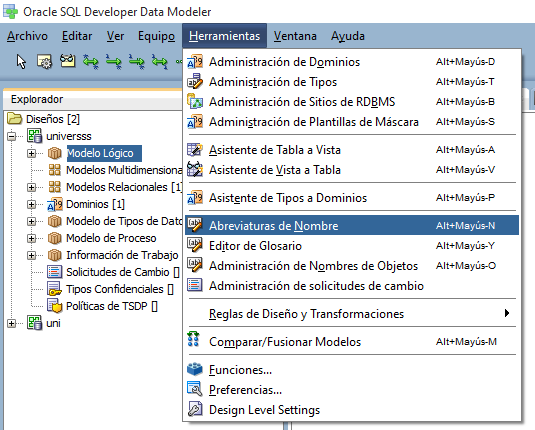
\includegraphics[width=11cm]{./images/5-1 Ejercicio 2/1.png}
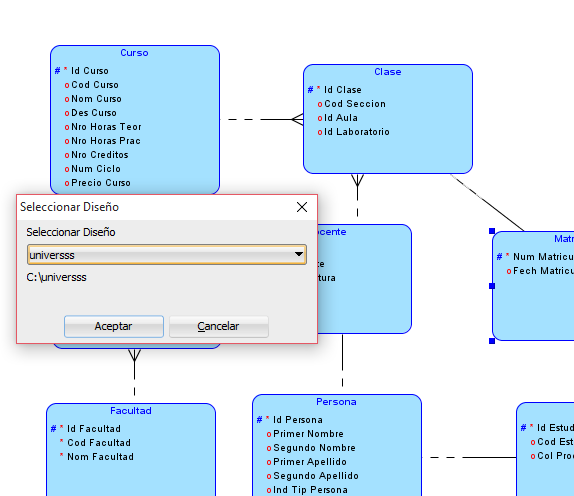
\includegraphics[width=11cm]{./images/5-1 Ejercicio 2/2.png}
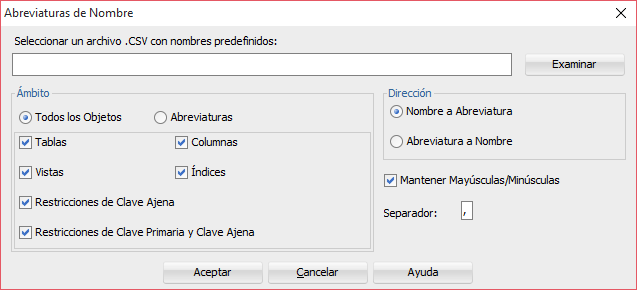
\includegraphics[width=14cm]{./images/5-1 Ejercicio 2/3.png}
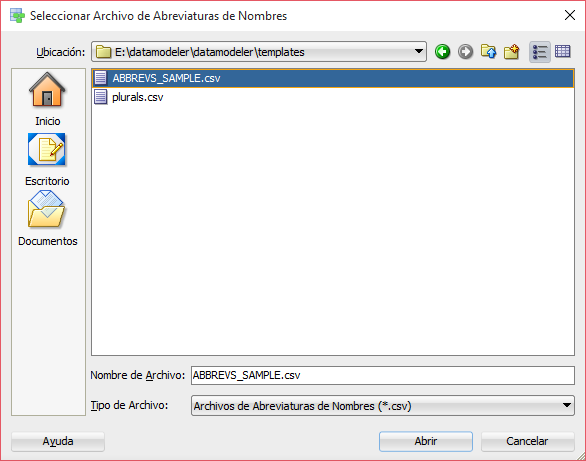
\includegraphics[width=11cm]{./images/5-1 Ejercicio 2/4.png}
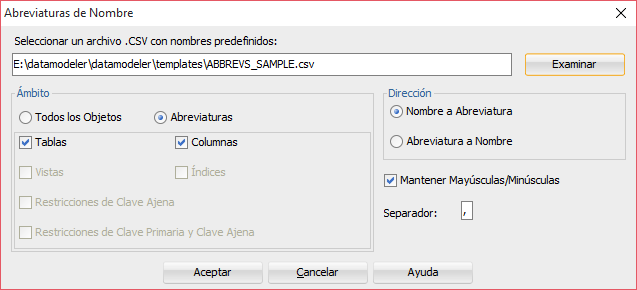
\includegraphics[width=11cm]{./images/5-1 Ejercicio 2/5.png}
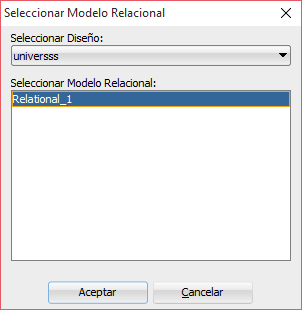
\includegraphics[width=7cm]{./images/5-1 Ejercicio 2/6.png}
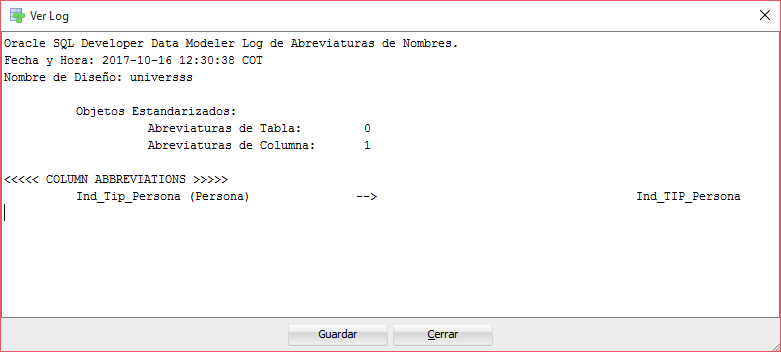
\includegraphics[width=14cm]{./images/5-1 Ejercicio 2/7.png}
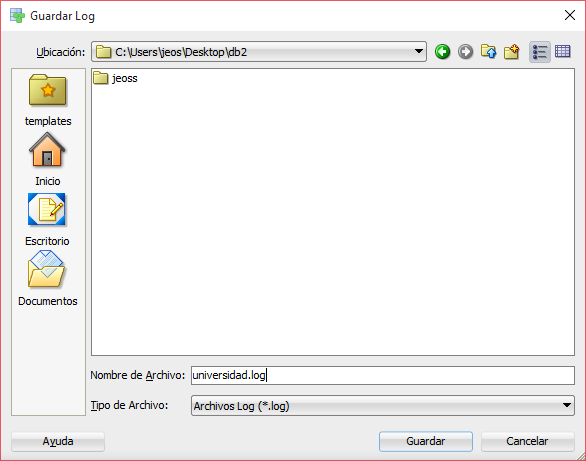
\includegraphics[width=11cm]{./images/5-1 Ejercicio 2/8.png}




\section{5-1 Ejercicio 3: Creación de un Juego de Reglas}\label{se:nudo}
\lhead[\thepage/\pageref{LastPage}]{\thesection. Nudo}
\rhead[\thesection. Nudo]{\thepage/\pageref{LastPage}}

Descripción general\\
En esta práctica, creará un juego de reglas para la base de datos académica.\\
Tareas\\
Para crear un juego de reglas, realice los siguientes pasos:\\
\begin{enumerate}

\item Seleccione Design Rules en el menú Tools.
\item Haga clic en el separador Rule Set y, a continuación, en el icono Add Rule Set (signo más).
\item Especifique un nombre para el grupo de reglas.
\item Haga clic en el icono de lápiz Rule Set Properties.
\item Utilice el cuadro de diálogo Rule Set Properties para mover las reglas deseadas de la columna All Rules a la columna Selected Rules.
\item Una vez realizada esta operación, seleccione "Apply Selected RuleSet" para aplicar el juego de reglas seleccionado al diseño actual
\end{enumerate}
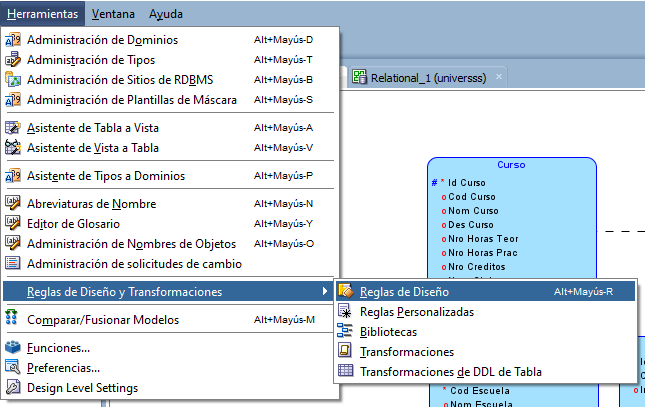
\includegraphics[width=11cm]{./images/5-1 Ejercicio 3/1.png}
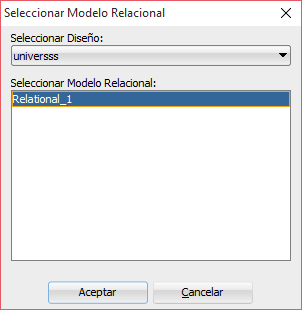
\includegraphics[width=10cm]{./images/5-1 Ejercicio 3/2.png}
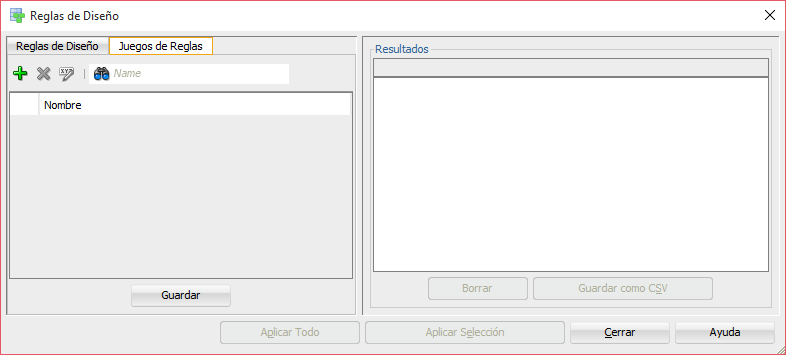
\includegraphics[width=11cm]{./images/5-1 Ejercicio 3/3.png}
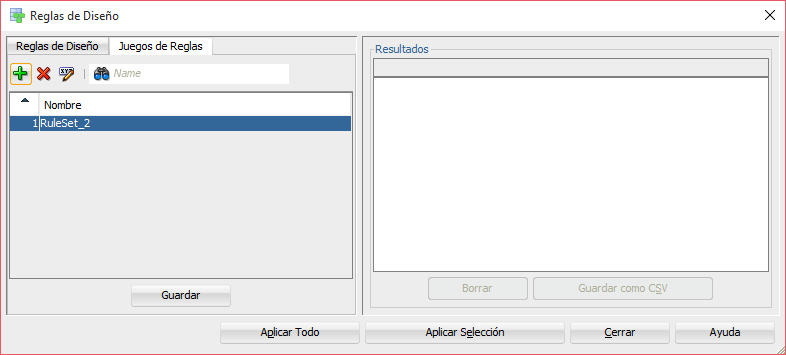
\includegraphics[width=11cm]{./images/5-1 Ejercicio 3/4.png}
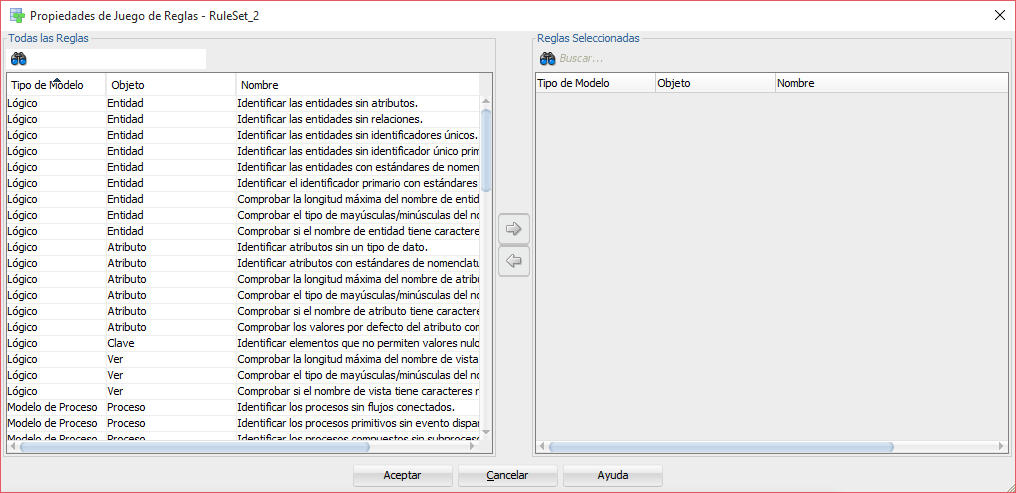
\includegraphics[width=11cm]{./images/5-1 Ejercicio 3/5.png}
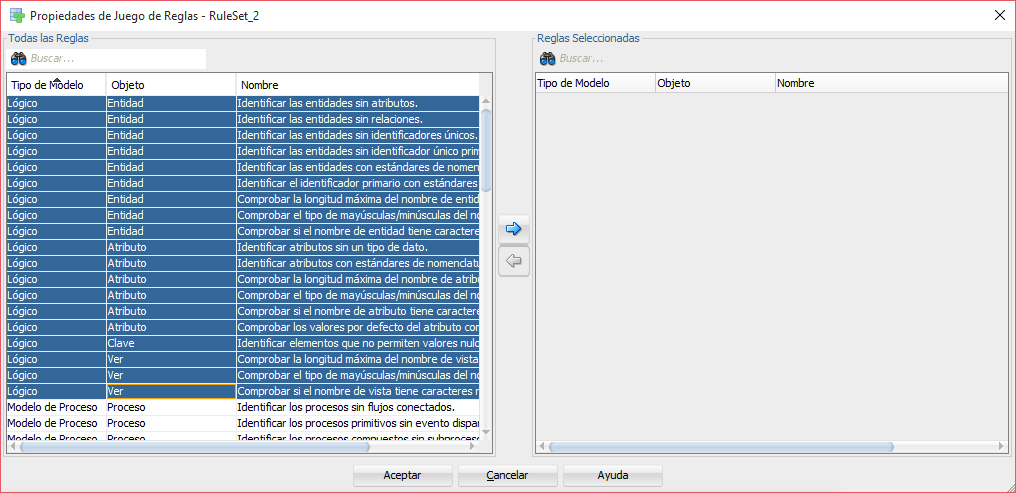
\includegraphics[width=11cm]{./images/5-1 Ejercicio 3/6.png}
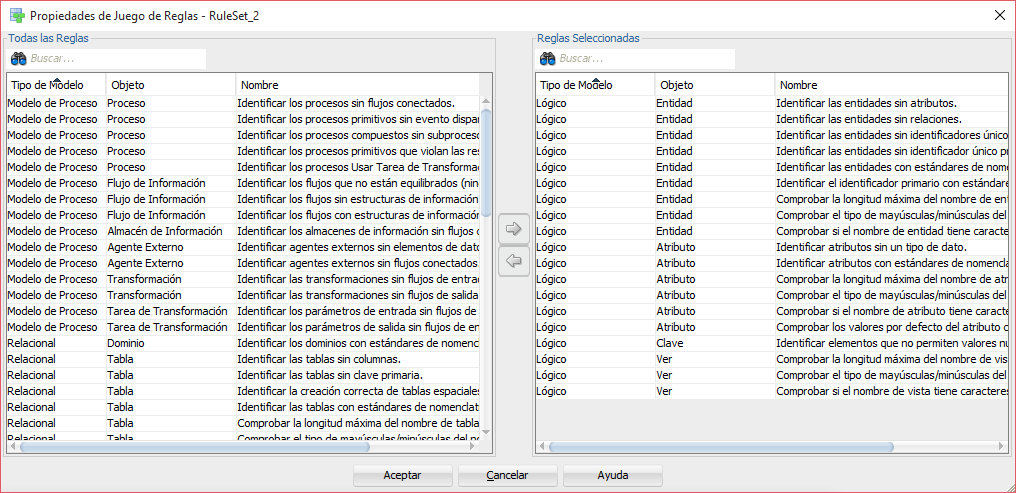
\includegraphics[width=11cm]{./images/5-1 Ejercicio 3/7.png}
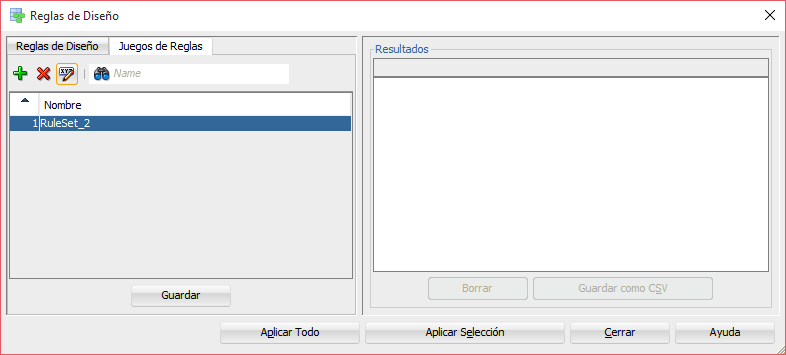
\includegraphics[width=11cm]{./images/5-1 Ejercicio 3/8.png}



\section{5-1 Ejercicio 4: Realización de Ingeniería Directa del Diseño para Aplicar el Glosario y el Estándar de Nomenclatura}\label{se:nudo}
\lhead[\thepage/\pageref{LastPage}]{\thesection. Nudo}
\rhead[\thesection. Nudo]{\thepage/\pageref{LastPage}}
Descripción general\\
En esta práctica, realizará ingeniería directa del diseño para aplicar el glosario y el estándar de nomenclatura.\\
Tareas\\
1. Para que el glosario se aplique durante la ingeniería, debe agregarlo en el cuadro de diálogo Preferences
de la página Naming Standard. Para asegurarse de que se aplica el glosario al realizar la ingeniería
directa del modelo, realice los siguientes pasos:\\
\begin{enumerate}
\item Haga clic con el botón derecho en el modelo Design en el explorador y seleccione Properties.
\item Amplíe Settings y haga clic en el nodo Naming Standard.
\item Haga clic en el icono “+” en la región Glossary y navegue hasta la ubicación del glosario.
\end{enumerate}
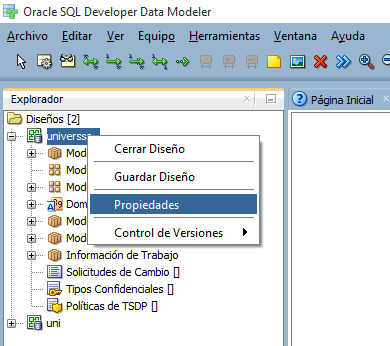
\includegraphics[width=11cm]{./images/5-1 Ejercicio 4/1.png}
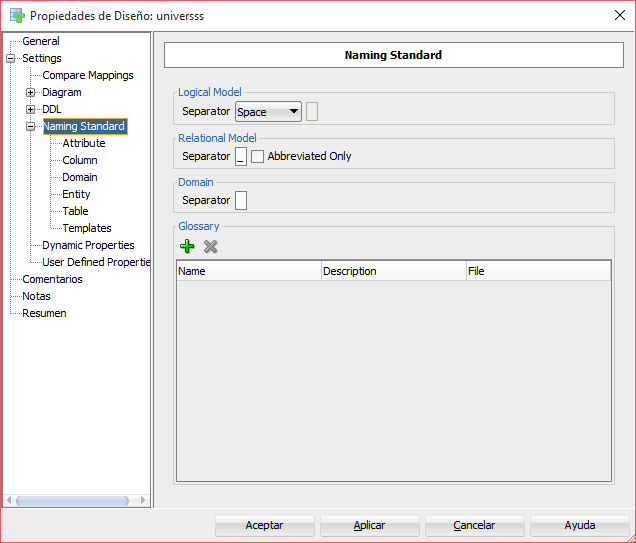
\includegraphics[width=11cm]{./images/5-1 Ejercicio 4/2.png}


\section{5-2 Ejercicio 1}\label{se:nudo}
\lhead[\thepage/\pageref{LastPage}]{\thesection. Nudo}
\rhead[\thesection. Nudo]{\thepage/\pageref{LastPage}}




\section{5-2 Ejercicio 2}\label{se:nudo}
\lhead[\thepage/\pageref{LastPage}]{\thesection. Nudo}
\rhead[\thesection. Nudo]{\thepage/\pageref{LastPage}}
\section{5-2 Ejercicio 3}\label{se:nudo}
\lhead[\thepage/\pageref{LastPage}]{\thesection. Nudo}
\rhead[\thesection. Nudo]{\thepage/\pageref{LastPage}}
\section{5-2 Ejercicio 4}\label{se:nudo}
\lhead[\thepage/\pageref{LastPage}]{\thesection. Nudo}
\rhead[\thesection. Nudo]{\thepage/\pageref{LastPage}}



\section{6-1 Ejercicio 1}\label{se:nudo}
\lhead[\thepage/\pageref{LastPage}]{\thesection. Nudo}
\rhead[\thesection. Nudo]{\thepage/\pageref{LastPage}}

\section{Desenlace}\label{se:des}
\lhead[\thepage/\pageref{LastPage}]{\thesection. Desenlace}
\rhead[\thesection. Desenlace]{\thepage/\pageref{LastPage}}

\bibliographystyle{acm} 
\bibliography{biblio}
\addcontentsline{toc}{section}{Bibliografía}
\lhead[\thepage/\pageref{LastPage}]{\thesection. Bibliografía}
\rhead[\thesection. Bibliografía]{\thepage/\pageref{LastPage}}

\end{document}
